\subsection{Development Process} \label{Development Process section}

In this section, we describe the progress on the artefact development, the detail for the experiments is given as Section \ref{Research Design section}.
For T1 - 2022, we aim to partly solve the research question (see Section \ref{Problem Section}) by implement a minimum viable artefact that contains a series of exploration experiments.
We summarise the experiment results from Section \ref{Result section} as the table \ref{Experiment summary table}.

\begin{table}
    \centering
    \begin{tabular}{|| c c c ||}
        \hline
        Ansatz   & Method                               & Variance of gradients \\[0.5ex]
        \hline \hline
        NLocal   & Default                              & Decay                 \\
        \hline
        TwoLocal & Default                              & Decay                 \\
        \hline
        NLocal   & Local Cost Function, Shallow circuit & Sustain               \\
        \hline
        TwoLocal & Local Cost Function, Shallow circuit & Sustain               \\
        \hline
    \end{tabular}
    \caption{
        The experiments that we implemented in the Python Notebook. We test the same ansatzes with different methods, we record the results as the vanishing rate of gradient when the number of qubits increased.
    }
    \label{Experiment summary table}
\end{table}

\almarginpar{How is the development process related to the research design and its process defined in Fig 9}
In more detail, the minimum viable artefact is a Python notebook file containing Python scripts to run the experiment.
We run the notebook with IBM Quantum Experience, as they provide online services for simulating quantum hardware.
This artefact outcome will not answer the research question completely.
However, it covers the first half of the experiment and ensures that the outcome is ready to advance to the next steps.
\almarginpar{You need to show that you have followed your research design}

\subsection{The Quantum Provider}
\almarginpar{Fault free runs are not exactly simulating the quantum device, any comment or justification? Perhaps future work? \\ - addressed}
For this experiment, we are using the quantum emulator provided by Qiskit.
The QASM simulator is used to mimic an IBMQ device.
Additionally, QASM simulator by default has no noise, so we can expect the result to be noise-free.
Note that the fault free emulators are not exactly reflecting the quantum devices as the actual devices may suffer from various types of noise.
However, considering the allowed time span for these experiments, we will use the QASM simulator for T1-2022 and leave the actual quantum devices for future works.


\subsection{Creating Ansatzes}
\almarginpar{Which of the ansatze would be most useful to support QNN? Wouldn't RealAmplitudes be useful for "real" QNN implementation?}
We have chosen two ansatzes \textit{NLocal} and \textit{TwoLocal} from the Qiskit circuit library due to their wide usage in quantum machine learning.
As discussed in the Research Design section \ref{Research Design section}, we configure the ansatz objects such that initially their gradient variances decrease exponentially with the number of qubits.
These characteristics are:
\begin{itemize}
    \item The circuit depth;
    \item The number of qubits to be measured for the cost function;
    \item The randomised parameters.
\end{itemize}

An example of circuits generated by Qiskit is visualised in Figure \ref{Ansatz samples}.
By altering the repetition number and qubit number, we can generate different ansatz.
The circuit depth is the largest number of gate operations across all qubit registers in a circuit.
Furthermore, as the circuit high-level definition is translated into the gate set available on a given quantum machine, the circuit depth may significantly increase.
Obviously, as the ansatz repetition grows, the circuit depth also grows.
Figure \ref{Ansatz samples} further shows that for a fully entangled ansatz, the higher number of qubits also leads to deeper circuit.

\begin{figure}
    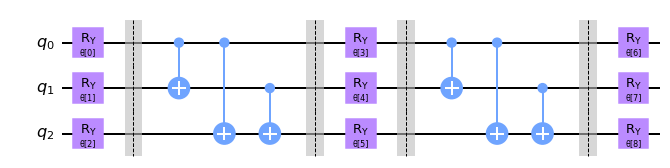
\includegraphics[width=\textwidth]{Artefact/Appendices/ansatz3-2.png}
    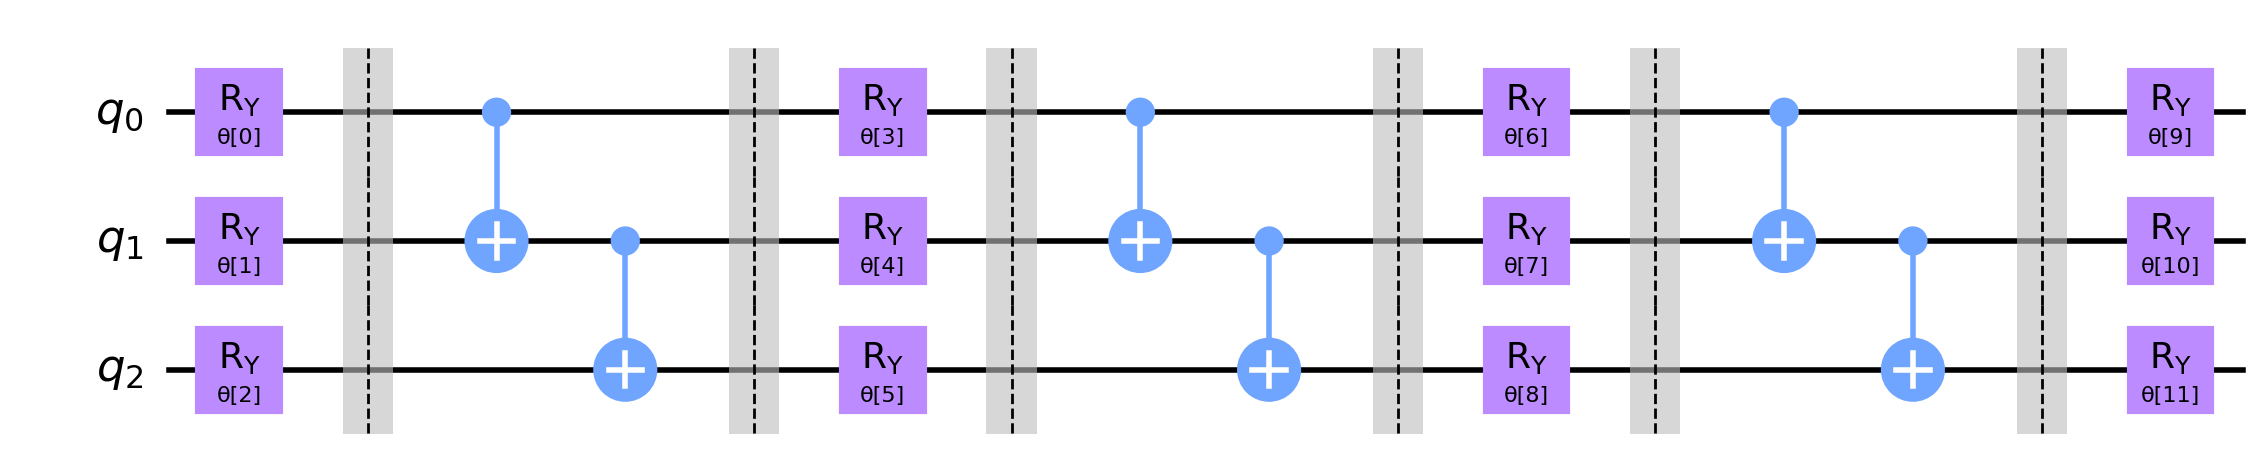
\includegraphics[width=\textwidth]{Artefact/Appendices/ansatz3-3.png}
    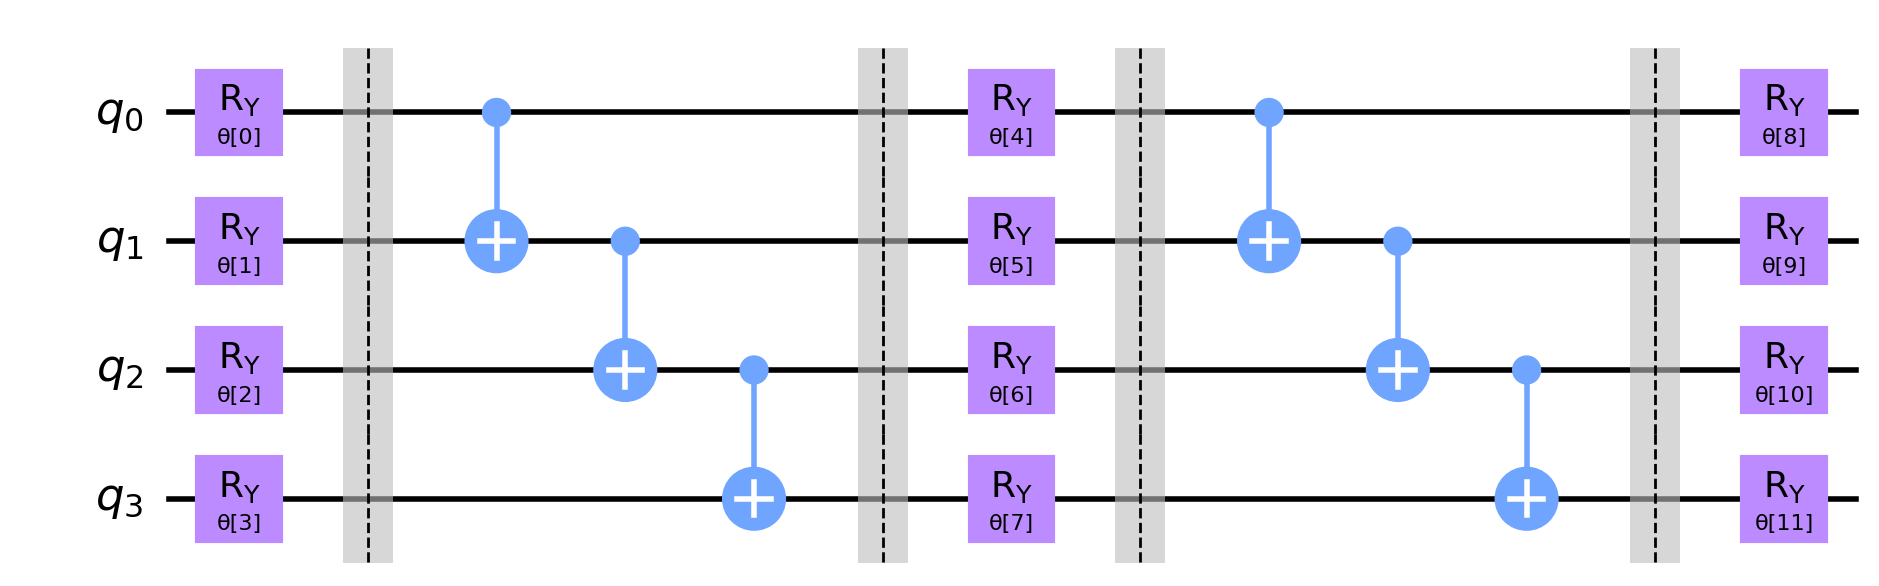
\includegraphics[width=\textwidth]{Artefact/Appendices/ansatz4-2.png}
    \caption{
        Samples of parameterised circuits generated by the Qiskit framework with 'full entanglement' option.
        The ansatz is a sequence of rotation layers and entanglement layers.
        Above: an ansatz of three qubits and two repetition layers.
        Middle: an ansatz of three qubits and three repetition layers.
        Below: an ansatz of four qubits and two repetition layers.
    }
    \label{Ansatz samples}
\end{figure}

\subsection{Visualise the Variance}
To calculate the gradient variance, we use the parameter shift rule from Eq. (\ref{Parameter-shift rules}) as implemented in Qiskit Gradient Framework.
The BP phenomena can be verified when the gradient variance decreases with an increased number of qubits and repetition layers.

To visualise the gradient variances, we have plotted a range of random parameters for each ansatz as the initial starting point.
Such randomised parameters are generated 100 times uniformly to calculate the gradients.
We then plot the variance values of the gradients for different numbers of qubits and repetition values for a range of 2 to 9 qubits and ansatz layer repetition.
Note that the neural network generated in this experiment is not designed to answer a problem, we will focus on the trainability of each method in later steps of the experiment.

In short, we use 100 uniformly randomised parameters to scan the gradient, then we calculate the "slope" of the gradient.

\subsubsection{Default Configurations for Ansatzes}
The ansatzes with default configuration will have unrestricted growth of circuit depth.
We implement the default ansatz to have the number of qubits and repetition increased iteratively.

\subsubsection{Local Cost Function and Shallow Depth Implementation}
\almarginpar{There is some repetition between the first and the second paragraph, improve!}
We implemented the \textit{Global Cost Function} as the measurement output for all qubits, while the \textit{Local Cost Function} is the measurement for the first two qubits.
Section \ref{Shallow Circuits, Local Cost Function section} and figure \ref{cost functions} previously explained the differences between the two cost functions.
The shallow ansatz is the same as compared with the default, however, the repetition number is kept as a constant number.